In cui si spiega nei dettagli lo sviluppo del componente di backend web, interfaccia unificata ai backend di scansione.

Come anticipato, il backend si interfaccerà esclusivamente con \textbf{Greenbone OpenVAS}.

\section{Virtual environment e gestione delle librerie}
In programmazione è fondamentale stabilire un ambiente di sviluppo ben strutturato e isolato. A tal fine, è stato utilizzato un \textbf{virtual environment}, comunemente abbreviato in \texttt{virtualenv}, pratica standard della gestione di progetti Python.

Un virtual environment è un ambiente isolato che consente di installare pacchetti Python senza influenzare il sistema globale o altri progetti. Questa pratica è considerata una buona norma nello sviluppo software, poiché garantisce che le dipendenze di un progetto siano gestite in modo indipendente, evitando conflitti tra librerie e versioni diverse. Inoltre, l'uso di un virtual environment facilita la riproducibilità del progetto, consentendo ad altri sviluppatori di configurare facilmente l'ambiente di lavoro con le stesse dipendenze. In questo caso il progetto è stato sviluppato singolarmente dall'autore di questo documento, ma la riproducibilità del progetto è comunque fondamentale in sede di deployment, come si vedrà in \ref{deployment-backend}.

Inizialmente, si è optato per l'uso di \textbf{Poetry}, un gestore di dipendenze e un sistema di packaging avanzato per Python che semplifica la gestione delle librerie e delle versioni. Poetry offre funzionalità avanzate, come la risoluzione automatica delle dipendenze e la creazione di un file di lock, che garantisce che le stesse versioni delle librerie siano utilizzate in tutti gli ambienti. Tuttavia, dopo una valutazione approfondita, si è deciso di passare a un approccio più semplice e comune, utilizzando un file \texttt{requirements.txt} per gestire le dipendenze del progetto. Questa scelta è stata motivata dalla volontà di ridurre la complessità e le astrazioni associate all'uso di Poetry, poiché le funzionalità aggiuntive offerte da quest'ultimo non erano state sfruttate nel contesto specifico del progetto. In particolare, Poetry è maggiormente indicato per la gestione delle dipendenze di \emph{codebase} utilizzate poi come librerie in altri progetti.

Il file \texttt{requirements.txt} è un formato standard per elencare le dipendenze di un progetto Python. In pratica esso è spesso realizzato automaticamente mediante la redirezione dell'output del comando \texttt{pip freeze}, che elenca tutte le dipendenze di progetto. Il file in questo modo contiene e specifica tutte le librerie richieste con le relative versioni, facilitando l'installazione delle stesse nei nuovi ambienti tramite il comando \texttt{pip install -r requirements.txt}. Questo approccio è ampiamente utilizzato nella comunità Python e risulta particolarmente efficace per progetti di dimensioni moderate, dove la gestione delle dipendenze non richiede funzionalità avanzate. Come questo progetto, che non sarà una libreria, ma piuttosto un semplice progetto \emph{standalone} con poche dipendenze di comodo.

\section{Controllo di versione}
Tutto il codice è stato manutenuto sotto \textbf{Git} come sistema di controllo versione (VCS: Version Control System). Git e altri strumenti simili sono fondamentali per la gestione del codice sorgente, poiché consentono agli sviluppatori di tenere traccia delle modifiche apportate al progetto nel tempo, ed eventualmente di annullarle, navigando tra le varie versioni del codice.

\section{Architettura dei package e del codice}
L'organizzazione del progetto Flask è stata adattata alle specifiche esigenze della REST API in questione, ottimizzando la struttura per garantire chiarezza e manutenibilità, rimuovendo le parti non necessarie. Per esempio, è stata omessa la cartella \texttt{templates/}, tipicamente utilizzata per i template Jinja nelle applicazioni web tradizionali, poiché non è necessaria in un contesto API, dove l'interazione avviene principalmente attraverso richieste e risposte in formato JSON.

Tutto il codice è stato collocato all'interno di un package Python denominato \texttt{gvmrest}, che rappresenta il nome del progetto. All'interno di questo package principale, sono stati creati tre ulteriori package: \texttt{blueprints}, \texttt{gmp} e \texttt{models}:

\begin{itemize}
    \item \texttt{blueprints} contiene i Blueprint di Flask, una funzionalità che consente di organizzare l'applicazione in moduli logici. Questa separazione aiuta a evitare la creazione di file troppo grandi e con poca coerenza interna, facilitando la gestione del codice e migliorando la leggibilità. I Blueprint permettono di raggruppare le route e le relative logiche in base ai domini dell'API, rendendo l'architettura più modulare e scalabile.
    \item \texttt{gmp} è dedicato alla gestione dell'autenticazione, comprendente funzionalità come login, logout e recupero dell'utente loggato, interfacciandosi con l'API di Greenbone OpenVAS tramite il protocollo GMP (Greenbone Management Protocol). Questo package funge da collante tra Flask e GMP, utilizzando la libreria \texttt{python-gvm} di Greenbone per facilitare le comunicazioni e le operazioni necessarie.
    \item Infine, il package \texttt{models} contiene la definizione delle entità, organizzate in file separati, che rappresentano il modello dei dati indotto dal protocollo GMP. Per quanto verbosa in termini di numero di file, questa struttura consente di mantenere il codice ben organizzato e facilmente estensibile, facilitando l'aggiunta di nuove entità o modifiche a quelle esistenti.
\end{itemize}

\begin{figure}
    \centering
    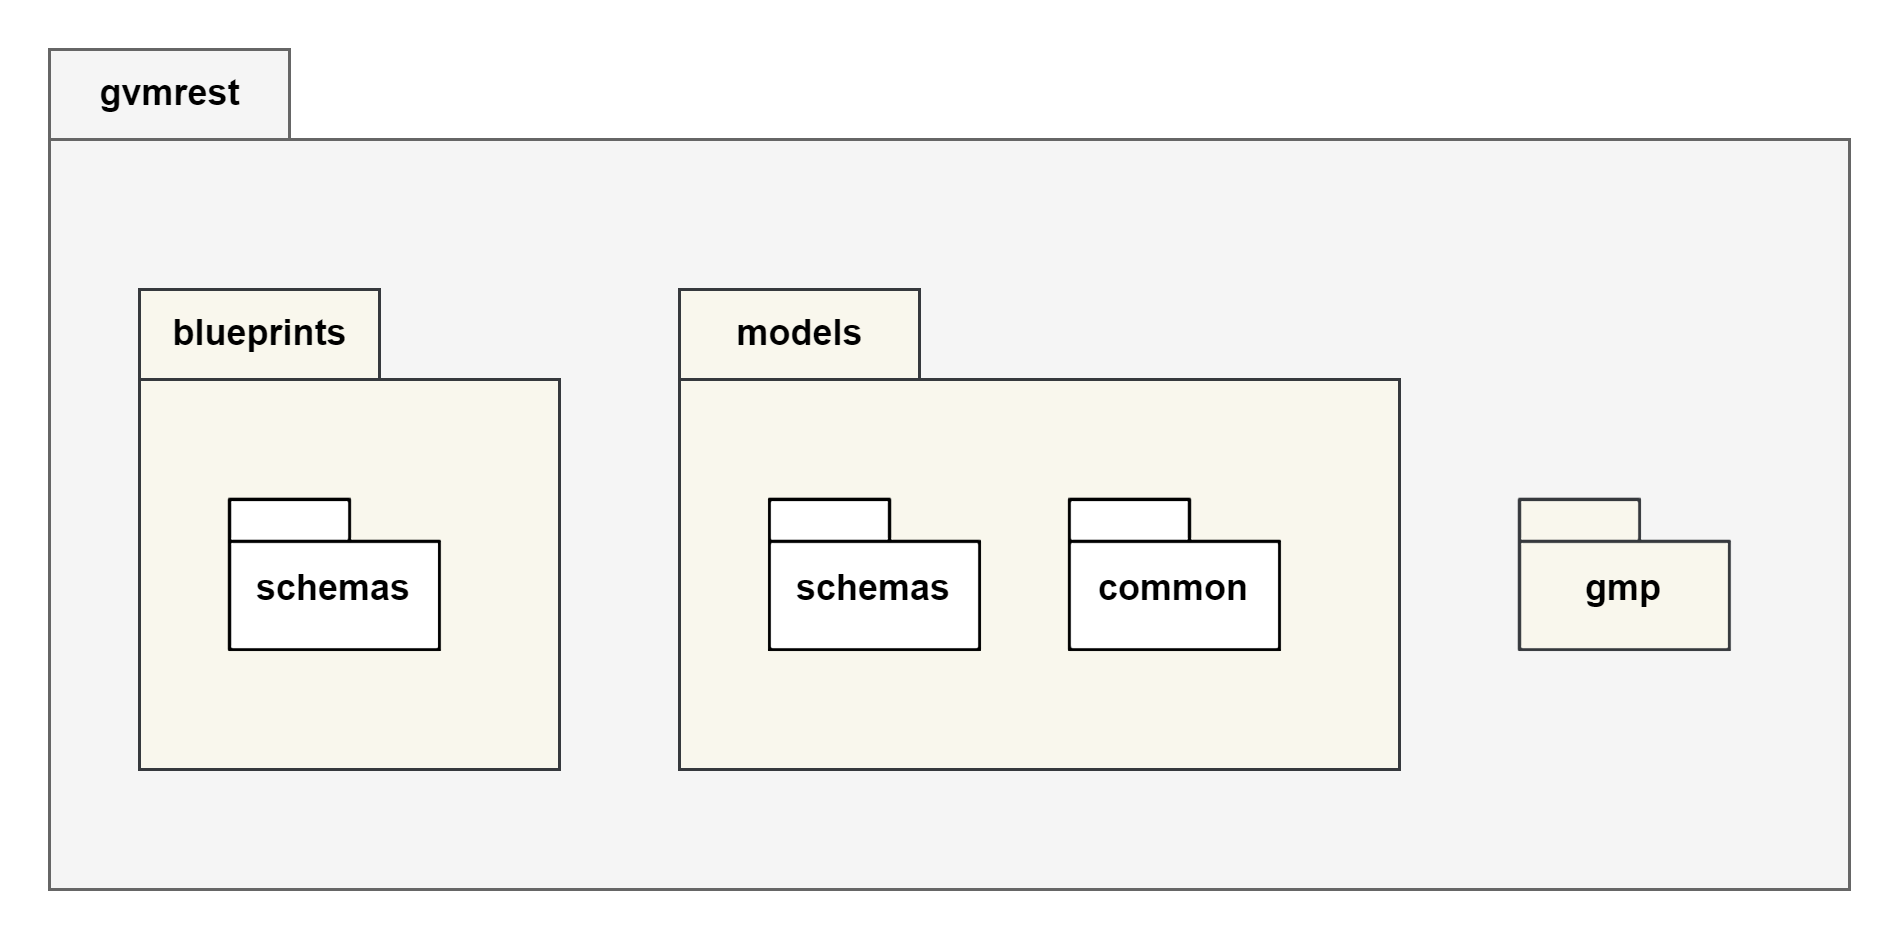
\includegraphics[width=0.8\textwidth]{img/packages.png}
    \caption{Diagramma dei package del backend Flask}
\end{figure}

\subsection{File di inizializzazione}
I file \texttt{\_\_init\_\_.py} di alcuni di questi package sono stati utilizzati in modo peculiare per ottimizzare la configurazione dell'applicazione:
\begin{itemize}
    \item Nel package principale \texttt{gvmrest} il file di \emph{init} implementa un'\emph{application factory} (o \emph{factory function}), un design pattern comune nei progetti Flask.

\begin{lstlisting}[caption={Application factory}]
def create_app():
    app = APIFlask(__name__)
    env = DotEnv(app)
    env.init_app(app)
    app.security_schemes = {
        'cookie': {
            'type': 'apiKey',
            'in': 'cookie',
            'name': 'session'
        }
    }
    app.config.from_mapping(
        SESSION_COOKIE_HTTPONLY=True,
        REMEMBER_COOKIE_HTTPONLY=True,
        SESSION_COOKIE_SAMESITE='Strict'
    )

    setup_server_side_sessions(app)

    from gvmrest import blueprints
    blueprints.register_into(app)

    CSRFProtect(app)

    setup_cors(app)

    return app
\end{lstlisting}

    \item Nel package di secondo livello, \texttt{blueprints}, l'inizializzazione contiene una funzione dedicata alla registrazione di tutti i Blueprint Flask contenuti nel package. Questo approccio consente all'\emph{application factory} di richiamare semplicemente questa funzione, evitando la necessità di enumerare singolarmente tutti i blueprint.

\begin{lstlisting}[caption={Registrazione dei blueprint}]
API_PREFIX = '/api'

def register_into(app: APIFlask):
    from .auth import bp, login_manager
    app.register_blueprint(bp, url_prefix=API_PREFIX + bp.url_prefix)
    login_manager.init_app(app)
    
    from .configs import bp
    app.register_blueprint(bp, url_prefix=API_PREFIX + bp.url_prefix)
    
    from .scanners import bp
    app.register_blueprint(bp, url_prefix=API_PREFIX + bp.url_prefix)

    ...
\end{lstlisting}
    
    In questo modo, il punto di variabilità si concentra esclusivamente nel file \texttt{\_\_init\_\_.py} del package, semplificando la manutenibilità e rendendo più agevole l'aggiunta o la rimozione di blueprint in futuro.
\end{itemize}

\subsection{Blueprint, REST API e MethodView}
L'uso di APIFlask implica la necessità di usare i Blueprint forniti dalla libreria, che sono di fatto un \emph{wrapper} attorno ai Blueprint Flask (chiamati \texttt{APIBlueprint}).

Per strutturare ancora di più il codice, si è cercato di fornire un'architettura similare a tutti i Blueprint dedicati a compiti simili. Infatti, quasi tutti i blueprint effettuano le classiche operazioni CRUD\footnote{Create, Read, Update, Delete: ovvero creare una risorsa, leggere una risorsa, aggiornare una risorsa, cancellare una risorsa} con vari gradi di completezza.

Flask mette a disposizione la classe \texttt{MethodView} proprio per questo caso. Si tratta di una classe che consente di gestire più metodi HTTP (ad esempio GET, POST, PUT, DELETE) all'interno di una singola classe. Ciò consente di organizzare il codice in modo più pulito e facile da mantenere.

Le MethodView sono utili quando si desidera gestire più azioni su una stessa risorsa in modo semantico (caratteristica chiave delle REST API), ad esempio:
\begin{itemize}
    \item Gestire una richiesta GET per recuperare i dati di una risorsa
    \item Gestire una richiesta POST per creare una nuova risorsa
    \item Gestire una richiesta PUT per aggiornare una risorsa esistente
    \item Gestire una richiesta DELETE per eliminare una risorsa
\end{itemize}

\begin{lstlisting}[caption={Blueprint API e MethodView con decoratori comuni}, basicstyle=\ttfamily\footnotesize\color{one-text}]
bp = APIBlueprint('users', __name__, url_prefix='/users')

class Users(MethodView):
    decorators = [login_required, bp.doc(security='cookie')]
    
    @bp.input(PaginatedUsersQuery, location='query')
    @bp.output(PaginatedUsers)
    def get(self, query_data: dict):
        data, total, pages = models.User.paginate(
            page=query_data['page'],
            filter_string='',
            sort=query_data['sort'],
            direction=query_data['direction']
        )
    
        return {
            'total': total,
            'page': query_data['page'],
            'pages': pages,
            'data': data
        }
    
    @bp.input(UserStoreRequest, arg_name='user')
    @bp.output(UserSchema, status_code=201)
    def post(self, user: dict):
        try:
            return models.User.create(user).__dict__, 201
        except GvmResponseError as e:
            return {
                'message': e.message
            }, int(e.status)
    
    
class User(MethodView):
    decorators = [login_required, bp.doc(security='cookie')]
    
    @bp.output(UserSchema)
    def get(self, user_uuid):
        try:
            return models.User.find(user_uuid).with_tasks()
        except GvmResponseError as e:
            return {'message': e.message}, int(e.status)
    
    @bp.output(ErrorMessageResponse, status_code=204)
    @bp.doc(responses=[404])
    def delete(self, user_uuid):
        try:
            models.User.delete(user_id=user_uuid)
            return '', 204
        except GvmResponseError as e:
            return {'message': e.message}, int(e.status)


bp.add_url_rule('', view_func=Users.as_view('users'))
bp.add_url_rule('/<uuid:user_uuid>', view_func=User.as_view('user'))
\end{lstlisting}

Le MethodView consentono anche di applicare globalmente i decoratori Python, definendoli come attributi d'istanza. Nel caso specifico, le nostre MethodView sono definite con i decoratori di Flask-Login, rendendo tutte le viste automaticamente protette dall'accesso non precedentemente autorizzato. Inoltre, con un ulteriore decoratore proprio di APIFlask è possibile segnalare le viste come protette dall'autenticazione, ottenendo questa informazione durante la generazione automatica della documentazione interattiva.

\subsection{Schemi Marshmallow}
Dalla scelta di utilizzare il meta-framework di APIFlask deriva anche la scelta obbligata della libreria di gestione degli schemi dei dati: Marshmallow (invece di Pydantic). APIFlask supporta di fatto solo Marshmallow, il che ha reso questa libreria una scelta naturale, anticipata già in \ref{design-marshmallow}.

Marshmallow si integra facilmente con Flask tramite appositi plugin, ma APIFlask offre una serie di automazioni che semplificano la validazione degli schemi in input (JSON) e l'auto-formattazione delle entità restituite in JSON. Queste automazioni includono il filtraggio e il parsing degli attributi sia in input che in output, permettendo conversioni basilari e avanzate, con la possibilità di utilizzare callback e hook astratti offerti dalle classi base di Marshmallow e personalizzabili nelle singole classi di schema attraverso override.

\begin{lstlisting}[caption={Esempio di schema Marshmallow con validazione},basicstyle=\ttfamily\footnotesize\color{one-text}]
def unique_username(username: str):
    response = g.gmp.get_users(filter_string=f'name={username}')
    if response.find('user') is not None:
        raise ValidationError('Username already exists')


class UserStoreRequest(Schema):
    name = fields.String(
        required=True,
        validate=[
            validators.Length(min=1, error='Please supply a name'),
            unique_username
        ]
    )
    password = fields.String(
        required=True,
        validate=validators.Length(min=1, error='Please supply a password')
    )
    role = fields.String(
        required=True,
        validate=validators.OneOf(['user', 'tenant'])
    )
    quota_id = fields.UUID(required=True)
    hosts = fields.String(load_default='',
                          example='192.168.1.42,192.168.1.200-220,a.com',
                          validate=validate_hosts_specification)
    hosts_allow = fields.Boolean(default=False)

    @post_load
    def split_hosts(self, data, **kwargs):
        data['hosts'] = [host for host in data['hosts'].split(',') if host != '']
        data['role'] = current_app.config.get(f"ROLE_{data['role'].upper()}")
        return data
\end{lstlisting}

Tuttavia, a differenza di Pydantic, Marshmallow non consente di utilizzare direttamente i tipi nativi di Python, ma richiede l'uso di classi wrapper specifiche della libreria. Questo introduce un certo livello di astrazione indesiderata, anche se i vantaggi dall'uso di Marshmallow superano gli svantaggi che porta il non usare una libreria di questo tipo.

Per ogni entità, è necessario definire uno schema Marshmallow. Questi schemi sono stati organizzati in file separati, tipicamente uno schema per file.

I file di schema sono stati raggruppati in due package \texttt{schemas/}, che si trovano sotto \texttt{models/} (dove sono specificate le entità e i modelli di business logic) e \texttt{blueprints/} (dove sono definiti i formati delle richieste API, che spesso sono lievemente diversi o semplificati rispetto ai dati reali, e delle risposte API, che possono utilizzare la paginazione e avvolgere i dati di base, rendendo insufficiente lo schema della singola entità in alcuni casi).

\section{ORM basato su GMP}
Una parte importante dello sviluppo è stata la creazione di un \textbf{ORM (Object-Relational Mapping)} basato sull'API di GMP.

\subsection{Razionale}
Un \textbf{ORM} è una tecnica che consente di interagire con un database utilizzando oggetti di programmazione, piuttosto che scrivere direttamente query SQL. Questo approccio semplifica la gestione dei dati, permettendo agli sviluppatori di lavorare con le entità come se fossero oggetti, senza doversi preoccupare della complessità delle operazioni di database sottostanti.

Nel nostro caso, la libreria \texttt{python-gvm} restituisce entità in formato XML, che alla fine è essenzialmente puro testo / stringa di caratteri. Per tradurre queste entità in JSON, è necessario effettuare un parsing. Tuttavia, una semplice conversione da XML in oggetti JSON non è sufficiente, poiché il servizio Python deve anche eseguire query sulle entità correlate fra loro da relazioni (ad es. come reperire i report generati da un task di scansione specifico). Per fare questo occorre che le entità siano in qualche modo ``intelligenti'', e una rappresentazione ``stupida'' di tipo testuale è scomoda oltre che inefficiente.

Stante così le cose si può comunque costruire direttamente le query al sistema Greenbone utilizzando il linguaggio Powerfilter descritto in \ref{powerfilter} (in questo contesto Powerfilter rappresenta in tutto e per tutto il linguaggio SQL). Tuttavia, questo approccio comporterebbe un'interazione diretta con il livello più basso, con i controller del pattern MVC (i blueprint Flask, in questo caso) che dovrebbero gestire direttamente la logica dell'applicazione. È preferibile mantenere questa logica all'interno dei modelli, che sono stati progettati proprio per questo scopo.

Le classi di modello implementano di conseguenza un ORM atipico e unico nel suo genere. Di solito, un ORM si interfaccia direttamente con un'istanza di database, solitamente usando internamente il linguaggio SQL; ma, nel nostro caso, l'ORM si connette invece a un database indirettamente esposto tramite un'API pubblicata su Socket UNIX (GMP e il linguaggio di query Powerfilter).

\subsection{Implementazione concreta}
In questo ORM ogni sua classe modello è creata a partire dal documento XML reperito da GMP, che rappresenta un numero qualsiasi di entità reperite dal sistema.

Questo documento XML ritornato dalla libreria è già un oggetto Python (un'istanza di \texttt{Element} della dipendenza \texttt{lxml}) che facilita il parsing e l'estrazione dei dati. In sostanza, questo oggetto rappresenta il documento in RAM, consentendo delle operazioni di ricerca e manipolazione giusto un po' più comode rispetto alla cruda manipolazione di testo. Tuttavia, questa flessibilità non è sufficiente e la rappresentazione è troppo semplice per i nostri scopi.

Ogni classe dell'ORM agisce nel medesimo modo: il costruttore della classe modello estrae il contenuto del documento XML utilizzando semplici query ai tag del documento (con l'API di \texttt{lxml}), sfruttando metodi nativi o interfacce XPath\footnote{XPath è un linguaggio di query avanzato utilizzato per navigare attraverso gli elementi e gli attributi di un documento XML, secondo logiche complesse e permettendo di selezionare nodi specifici in modo altamente flessibile ed efficiente.}.

\begin{lstlisting}[caption={Destrutturazione dal documento XML a Python}]
class User(Authenticable):
    id: uuid.UUID
    name: str
    role_id: uuid.UUID
    role: str
    comment: str
    created: str
    owner: str
    hosts: dict
    quota: dict
    tags: list[Tag]
    in_use: bool

    def __init__(self, get_users_response: etree.Element):
        self.tasks = []
        user_tag = get_users_response.find('user')
        self.id = user_tag.attrib['id']
        self.name = user_tag.find('name').text
        self.role_id = user_tag.find('role').attrib['id']
        self.role = self._role_human(self.role_id)
        self.comment = user_tag.find('comment').text
        self.created = user_tag.find('creation_time').text
        self.owner = user_tag.find('owner/name').text
        self.hosts = {
            'allow': not bool(int(user_tag.find('hosts').attrib['allow'])),
            'exclusions': user_tag.find('hosts').text
        }
        self.in_use = bool(int(user_tag.find('in_use').text))

        tags = get_users_response.find('user/user_tags')
        tags = [] if tags is None else tags.xpath('tag')
        self.tags = [Tag(tag) for tag in tags]

        self.quota = self.get_month_quota()
    
    ...
\end{lstlisting}

Questa procedura consente di realizzare una prima traduzione da XML a un oggetto Python specifico per l'entità rappresentata (\texttt{Task}, \texttt{Report}, eccetera). A questo punto, ogni classe può offrire metodi specifici che astraggono l'interazione con le altre entità e, indirettamente, con il database. Di fatto si crea un ORM, ma astraendo qualcosa di più specialistico rispetto al più comune caso di un database SQL direttamente controllato da noi.

In questo modo, i controller (blueprint nel nostro caso) rimangono snelli e focalizzati, mentre il codice di basso livello e l'accesso ai dati sono segregati nei modelli e organizzati in metodi separati. Questo approccio per quanto inusuale aumenta la coerenza e riduce l'accoppiamento, migliorando in modo decisivo la manutenibilità e la chiarezza del codice. Non solo, la separazione del codice di accesso ai dati in metodi distanti favorisce e incoraggia anche un riuso del codice che non sarebbe altresì possibile.

\subsection{API generica / paginazione}
Nell'implementazione dell'ORM, sono stati creati metodi generici per facilitare la frequente interazione con le entità restituite dalla API GMP. Poiché queste entità sono quasi sempre restituite paginate in partenza, è fondamentale gestire la paginazione a livello di superclasse.

La classe \texttt{Model}, che funge da superclasse per tutte le classi di modello, implementa due metodi principali per l'interazione con il database:
\begin{itemize}
    \item \texttt{all()}: questo metodo restituisce tutti i record di un determinato modello, ``paginati'' di default, insieme al numero totale di record disponibili (non solo quelli nella pagina corrente). \texttt{all()} accetta anche una \texttt{filter\_string} definita in Powerfilter, che gestisce effettivamente la paginazione. È decorato come \texttt{@abstractmethod}, il che significa che l'implementazione specifica deve essere fornita dalle sottoclassi concrete. Tuttavia, l'idea è che \texttt{all()} non venga utilizzato direttamente, ma solo attraverso l'altro metodo di questa classe.
    \item \texttt{paginate()}: Questo metodo concreto riceve tutti i parametri relativi alla paginazione, come il numero di pagina, il numero di oggetti per pagina, l'ordinamento (ascendente o discendente e su quale attributo) e il filtraggio (gestito tramite una \texttt{filter\_string} in Powerfilter). \texttt{paginate()} esegue i calcoli necessari per determinare la pagina e costruisce una nuova \texttt{filter\_string} decorando quella iniziale con i valori necessari per gestire la paginazione. Questa \texttt{filter\_string} viene poi passata a \texttt{all()}, che recupera i record appropriati. Il metodo \texttt{paginate()} restituisce quindi i record paginati, insieme a informazioni utili per il frontend, come il numero totale di pagine e il numero totale di record.
\end{itemize}

\begin{lstlisting}[caption={Modello base dell'ORM}]
class Model:
    def __repr__(self):
        import pprint
        return pprint.pformat(self.__dict__)

    @classmethod
    def paginate(cls,
                 page: int,
                 filter_string: str,
                 rows: int = 20,
                 sort: str = None,
                 direction: str = 'asc'
                 ) -> tuple[list['Model'], int, int]:

        first = (page - 1) * rows + 1

        sort_kw = 'sort' if direction == 'asc' else 'sort-reverse'
        sort_query = None if sort is None else f'{sort_kw}={sort}'
        filter_string = filter_string + f" first={first} rows={rows} " + sort_query

        models, total = cls.all(filter_string=filter_string)

        pages = math.ceil(total / rows)

        return (
            models,
            total,
            pages
        )

    @classmethod
    @abstractmethod
    def all(cls, filter_string: str) -> tuple[list['Model'], int]:
        pass
\end{lstlisting}

Inoltre, la classe \texttt{Model} implementa anche il \emph{magic method} \texttt{\_\_repr\_\_()}, fornendo un'implementazione di default per la stampa in ambiente CLI. In particolare, l'implementazione usa \texttt{pprint} per stampare la rappresentazione interna a dizionario dell'oggetto, risultando particolarmente utile durante il debug o i test.

Per gestire la definizione di classi e metodi astratti, è stata necessariamente utilizzata la libreria \textbf{ABC (Abstract Base Classes)} di Python\footnote{Python non supporta le classi astratte a livello di linguaggio.}. Questa libreria consente di definire classi base astratte e metodi astratti, fornendo un modo per garantire che le sottoclassi implementino determinati metodi, mantenendo così una struttura coerente nell'ORM.

\subsection{Deserializzazione}
Il processo di deserializzazione da XML a oggetto Python inizia quando i costruttori delle classi modello ricevono un'istanza del documento XML in memoria, che, come già detto poco sopra, viene decomposto in attributi d'istanza del nuovo oggetto, convertendo i valori estratti in una rappresentazione nativa di Python.

I valori ovviamente necessitano di \emph{casting}, siccome la rappresentazione XML è puramente testuale, ma anche di una gestione del valor nullo e dell'assenza di valore. È comune infatti che alcuni valori siano del tutto assenti nel documento XML. In questi casi, si considera il tipo di riferimento come \emph{nullable}, utilizzando un tipo unione con il \texttt{None} di Python. Questo approccio consente di gestire in modo efficace i dati incompleti, dichiarando nell'interfaccia il rischio di inconsistenza, similarmente all'approccio usato da linguaggi come TypeScript o Kotlin. Questo viene fatto mediante le \texttt{type hint}, largamente usate in questo progetto. Questo non solo aiuta a mediare la natura dinamica di Python, ma fornisce anche un supporto migliore per le funzionalità di autocomplete negli IDE.

In generale, le classi concrete che rappresentano i modelli sono simili a una \emph{dataclass} di Python, poiché si concentrano principalmente sulla memorizzazione dei dati. Tuttavia, alcune di queste classi esibiscono anche comportamenti più ricchi grazie all'aggiunta di metodi specifici, che permettono di eseguire operazioni più complesse o di interagire con altre entità in modo meno ripetitivo e ridondante.

\subsection{Serializzazione}
Quando gli oggetti devono essere restituiti nella risposta della API, questi vengono semplicemente restituiti così come sono, senza nessuna particolare operazione. La presenza dei valori negli attributi della classe e lo schema Marshmallow fa sì che il processo di serializzazione sia assolutamente automatico, con lo schema Marshmallow che specifica cosa viene fatto passare della classe e secondo quale formato\footnote{Si noti che lo standard JSON non supporta numeri decimali, che vengono quindi restituiti come stringhe di caratteri. La conversione verrà gestita dal frontend.}.

\section{Quality of Detection}
Pur essendo un attributo specifico di OpenVAS si è voluto inserire comunque il QoD (già descritto precedentemente in \ref{qod}) nell'interfaccia dell'API, anticipando un eventuale parametro generico che identifichi l'affidabilità dei risultati, indipendente dal backend di scansione.

Questo parametro viene fornito all'API in tutte le richieste di risorse con paginazione, che di fatto sono le uniche che possono usare il valore di QoD per filtrare i risultati.

\section{Gestione delle schedule}
Le schedule sono gestite internamente da OpenVAS come delle stringhe in formato iCalendar, più alcuni metadati usati per la loro identificazione.

\subsection{iCalendar}
\textbf{iCalendar} è un formato standard per la rappresentazione di informazioni relative a eventi, appuntamenti e attività. È utilizzato per scambiare dati di calendario tra diverse applicazioni e servizi. Il formato è definito nella specifica RFC 5545 \cite{rfc5545} e consente di creare file con estensione \texttt{.ics}, che possono contenere dettagli come:
\begin{itemize}
    \item Data e ora di inizio e fine di un evento
    \item Fuso orario
    \item Descrizione dell'evento
    \item Luogo
    \item Informazioni di contatto
    \item Ripetizioni (per eventi ricorrenti)
    \item Allerta e promemoria
\end{itemize}
Questo formato è utile anche per specificare calendari che possono essere importati o condivisi tramite applicazioni come Outlook, Google Calendar o altre.

Per quanto riguarda il caso in esame, OpenVAS si serve di questo formato esclusivamente per specificare le scansioni che devono essere fatte in accordo con la schedule in oggetto, di fatto limitandosi alle seguenti informazioni:
\begin{itemize}
    \item Data e ora di inizio e fine scansione
    \item Ripetizioni per eventi ricorrenti
    \item Fuso orario
\end{itemize}

L'uso di un formato standard ovviamente semplifica lo sviluppo poiché ci si può appoggiare a librerie che automatizzano il processo di parsing e generazione di stringhe aderenti al formato iCalendar. Addirittura la documentazione stessa di \texttt{python-gvm} suggerisce l'uso della libreria \texttt{icalendar} di Python, e così si è fatto nel progetto in esame.

\begin{lstlisting}[caption={Uso di icalendar}]
icaltext = schedule_xml.find('icalendar').text
cal = Calendar()
self._ical = cal.from_ical(icaltext)
subcomp = self._ical.subcomponents[1]
dt_from: datetime.datetime = subcomp['dtstart'].dt
self.start = dt_from.isoformat()
self.duration = subcomp['duration'].dt.total_seconds()
self.dtstamp = subcomp['dtstamp'].dt.isoformat()
self.freq = subcomp['rrule']['freq'][0] if 'rrule' in subcomp else 'ONCE'
\end{lstlisting}

L'uso dello standard iCalendar è tornato utile anche in fase di standardizzazione dell'interfaccia dei dati in uscita, mantenendo il formato delle \texttt{RRULE} di iCalendar per descrivere il tipo di ricorrenza delle schedule.

\section{Autenticazione}
\subsection{Autenticazione con l'API Flask}
L'autenticazione degli utenti nell'API Flask è gestita utilizzando \textbf{Flask-Login}, una delle librerie più affidabili e popolari dell'ecosistema Flask. Questa libreria semplifica notevolmente il processo di autenticazione, implementando un sistema basato su cookie per gestire le sessioni degli utenti.

Flask-Login automatizza gran parte delle operazioni di login e logout, fornendo metodi semplici e intuitivi per eseguire queste funzioni quando necessario. Inoltre, la libreria offre un decoratore \texttt{@login\_required}, che consente di proteggere immediatamente e facilmente qualsiasi metodo-vista di Flask, garantendo che solo gli utenti autenticati possano accedervi.

Un aspetto fondamentale di Flask-Login è la necessità di fornire un metodo che restituisca l'oggetto utente corrispondente a un identificativo specifico. Questo metodo deve restituire l'oggetto utente se l'identificativo è valido, oppure None se non lo è. L'identificativo utilizzato è a discrezione del programmatore, così come la classe utente, purché vi sia coerenza interna nel sistema.

Nel contesto di questo progetto, è stato scelto di utilizzare l'ID dell'utente fornito dall'API GMP come identificativo. Questo ID è un UUID, in linea con il formato utilizzato per tutte le altre risorse interne al sistema GVM. Per rappresentare l'utente, è stata utilizzata la classe di modello che corrisponde alla risorsa utente di GMP, garantendo così una gestione coerente e integrata delle informazioni relative agli utenti.

\begin{lstlisting}[caption={User loader di Flask-Login}]
login_manager = LoginManager()

@login_manager.user_loader
def load_user(user_id: str):
    gmp = get_gmp()
    if gmp is None:
        return None
    res = gmp.get_user(user_id)
    return User(res)
\end{lstlisting}

\subsection{Autenticazione con l'API GMP}
L'autenticazione dell'applicazione Flask con l'API sottostante di GMP ha rappresentato invece una sfida complessa e delicata, come quasi tutti i casi in cui un'applicazione deve interagire in modo sicuro con un sistema di terze parti che non è ben configurato in tal senso (ad esempio, supportando OAuth).

Segue un'analisi delle problematiche riscontrate e dell'analisi effettuata di varie soluzioni applicative prima di giungere alla soluzione che è stata effettivamente adottata nel progetto.

\subsubsection{Requisiti}
Innanzitutto, si vuole che la sessione dell'utente loggato mantenga una connessione con l'API di GMP in background. Ma questo non è un compito banale. Le connessioni HTTP sono, per loro natura, \emph{stateless}, mentre l'API di GMP opera su una socket UNIX, che è intrinsecamente \emph{stateful} rispetto alle richieste HTTP in arrivo.

La connessione con l'API di GMP viene stabilita aprendo una socket UNIX e fornendo immediatamente le credenziali dell'utente, ovvero nome utente e password. Questo approccio consente di eseguire tutte le operazioni successive con i privilegi dell'utente autenticato.

\subsubsection{Pooling di connessioni}
Una possibilità può essere mantenere viva questa connessione in memoria tra le chiamate HTTP; ma questo è problematico, poiché i server web operano in modalità di parallelismo. Ad esempio, Gunicorn, il server web utilizzato per il deployment, gestisce le richieste in ingresso creando una serie di processi \emph{worker}, i quali non condividono la memoria RAM. Di conseguenza, mantenere le connessioni alla socket in memoria porterebbe a errori di tipo \emph{time-dependent}: una richiesta potrebbe avere successo solo se viene gestita da quel particolare \emph{worker} che ha tenuto in memoria la connessione, altrimenti fallirebbe.

\subsubsection{Multiprocessing / multithreading}
Sebbene Gunicorn consenta di precaricare un pezzo di codice e di fare il \emph{fork} dei processi worker successivamente, questo approccio garantisce solo che il pool di connessioni parta dallo stesso stato iniziale, senza assicurare coerenza nelle operazioni successive. Un'alternativa sarebbe implementare soluzioni di multiprocessing o multithreading. Tuttavia, il multiprocessing richiede lo scambio di messaggi e strutture dati tra processi, e le connessioni a socket UNIX non sono facilmente serializzabili con nessuna delle strategie di \emph{marshalling} comuni nell'ecosistema Python.

D'altra parte, il multithreading richiederebbe di configurare i worker di Gunicorn con GEvent, trasformando il server web in un singolo processo con più thread. Questo approccio, però, introduce la necessità di gestire sezioni critiche (per la gestione del pool delle connessioni) e meccanismi di sincronizzazione, come i semafori, di fatto compromettendo le performance. Tuttavia, ciò comporta un ulteriore problema: una singola connessione UNIX non può essere "multiplexata" e può rispondere a un solo comando alla volta. Anche con l'implementazione di sezioni critiche e semafori, le richieste simultanee sarebbero ingestibili.

\subsubsection{Gestione delle credenziali di terze parti}
In sintesi, l'unica soluzione praticabile per evitare di richiedere all'utente di inserire nome utente e password ad ogni chiamata API (un approccio di fatto estremamente scomodo e impraticabile) è quella di memorizzare in RAM il nome utente e, purtroppo, la password. Questo consente di ricreare le connessioni con la socket UNIX per ogni chiamata, garantendo la massima performance e soprattutto, scongiurando problemi di consistenza dei dati o dipendenze dalla rete, che sarebbero altresì inevitabili.

Questo approccio, per quanto sub-ottimo dal punto di vista delle buone pratiche di security, come si è visto è di fatto necessario per realizzare il sistema in oggetto.

Per mitigare il più possibile questa soluzione si sono introdotti tutta una serie di accorgimenti:
\begin{itemize}
    \item Le credenziali di terze parti sono salvate in sessione, ma rese \emph{server-side} rispetto al default \emph{client-side} di Flask.
    \item Le sessioni \emph{server-side} sono salvate in un'istanza di Redis, resa accessibile solo dalla rete interna di Docker Compose ed è pertanto inaccessibile da al di fuori della macchina. Internamente alla macchina invece è necessario disporre dei permessi di \texttt{root} per accedervi.
    \item Un'istanza di \textbf{Fernet} è generata e condivisa tra tutti i processi mediante il precaricamento di Gunicorn, efficace in questo caso visto che l'istanza non cambia nel tempo. Fernet è un sistema di crittografia simmetrica che fa parte della libreria di crittografia \texttt{cryptography} in Python, e di fatto implementa AES in modalità CBC.
    
    Grazie a Fernet le password sono crittografate prima di essere salvate su Redis. Chiaramente è meno sicuro di un hash, ma le hash impediscono il recupero della password che in questo caso è purtroppo necessario.
    \item La password usata da AES è generata casualmente al momento della creazione del server Gunicorn e non è mai salvata su disco o stampata a schermo, di fatto rimanendo solo nella RAM della macchina. Questo significa che ad ogni riavvio del server la password è scelta di nuovo e sessioni esistenti diventano invalidate.
\end{itemize}

\subsection{Proxying dell'API GMP}
Flask supporta l'uso di un oggetto ``globale'' per tutta la durata della richiesta web, chiamato semplicemente \texttt{g}. Questo oggetto è usato per riferirsi alla connessione con l'API GMP (in un'applicazione web maggiormente classica conterrebbe probabilmente un riferimento alla connessione con il database SQL), usando un metodo \texttt{get\_gmp()} che di fatto implementa un design pattern di tipo \emph{Proxy}.

\begin{lstlisting}[caption={Metodo proxy per la connessione GMP}]
def get_gmp() -> None | GMPv224[Any] | GMPv225[Any]:
    if 'gmp' not in g:
        g.gmp = Gmp(
            connection=UnixSocketConnection(path=current_app.config.get('GVMD_SOCKFILE')),
            transform=EtreeCheckCommandTransform()
        ).__enter__()
        try:
            g.gmp.authenticate(
                fernet.decrypt(session['name']).decode(),
                fernet.decrypt(session['password']).decode()
            )
        except InvalidToken as _:
            return None

    return g.gmp
\end{lstlisting}

Nello specifico, quando questo metodo viene invocato esso verifica se l'istanza di GMP è già presente, ovvero, se la connessione è stata già stabilita:
\begin{itemize}
    \item Se sì, ritorna la connessione già stabilita.
    \item In caso contrario è necessario stabilire una nuova connessione. La libreria \texttt{python-gvm} è usata per connettersi alla socket UNIX. Quindi, vengono reperite dalla sessione Redis le credenziali dell'utente, decriptate e infine usate per autenticare la connessione.
\end{itemize}

Infine, quando il flusso di richiesta / risposta web si conclude l'istanza Flask chiude la connessione manualmente, siccome (come già detto precedentemente) non è possibile fare \emph{pooling} di queste connessioni per ottimizzare le risorse del server.

\begin{lstlisting}[caption={Metodo di chiusura delle connessioni GMP}]
def close_gmp(e=None):
    gmp = g.pop('gmp', None)

    if gmp is not None:
        gmp.__exit__(None, None, None)
\end{lstlisting}

\begin{lstlisting}[caption={Aggancio per chiudere le connessioni}]
from .gmp import close_gmp
app.teardown_appcontext(close_gmp)
\end{lstlisting}

\section{Quota di scansione}
\subsection{Definizione del valore massimo}
La quota di scansione come detto è stata gestita mediante il sistema di tagging interno a Greenbone. In particolare, ogni utente riceve un tag di nome \texttt{quota:total} con come valore il numero di scansioni massime consentite per ogni mese. Questo tag è specificato al momento della creazione dell'utente da parte dell'utenza di livello superiore.

\subsection{Calcolo della quota consumata}

\begin{lstlisting}[caption={Calcolo della quota consumata (ad alto livello)}]
def get_consumed_quota(self, at: datetime):
    next_month = at + relativedelta(months=1)

    self.hosts_for_target = {}
    targets, _ = Target.all(filter_string=f'owner={self.name}')
    for target in targets:
        self.hosts_for_target[target.id] = target.max_hosts

    total_hosts = self.sum_past_reports_consumption(at, next_month)
    total_hosts += self.sum_scheduled_tasks_consumption()

    return total_hosts
\end{lstlisting}

La quota consumata è calcolata sommando i contributi di due parti:
\begin{itemize}
    \item Le scansioni passate in questo mese, usando i report delle scansioni\footnote{Per tenere sotto controllo l'occupazione del disco i report sono cancellati a rotazione. Ovviamente, il valore di \emph{turnaround} è stato scelto in modo tale da non compromettere la correttezza del precedente calcolo.} per determinare il numero di host coinvolti ogni volta (che non dipende da quanti host fossero attivi o meno al momento della scansione).
    \item Le scansioni future di questo mese, ovvero quelle pianificate / ricorrenti. Queste sono determinate con l'uso di una libreria Python specializzata, \texttt{recurring\_ical\_events}, che garantisce una gestione facilitata degli eventi ricorrenti definiti con standard iCalendar. Non avendo ancora rapporti, per contare l'impatto della scansione della quota si usa il bersaglio configurato.
\end{itemize}
Questa quota è quindi definita come attributo d'istanza dell'utente.

\subsection{Controllo della quota consumata}
La quota è controllata al momento dell'aggiunta di un task di scansione. In particolare, nel backend è stato definito un endpoint che verifica se il task passato nella richiesta API è accettabile per la quota fornita, oppure no. Per farlo opera in modo diverso a seconda del task specificato:
\begin{itemize}
    \item Se il task è configurato per l'esecuzione immediata allora questo è controllato esclusivamente rispetto alla quota disponibile di questo mese.
    \item Se invece il task è configurato per un esecuzione periodica allora la quota è controllata per ogni mese futuro, fermando i controlli con un'orizzonte temporale di un anno dal momento della creazione.
\end{itemize}
In questo modo la quota valida è controllata a monte dell'unica operazione che può intaccarla, così da garantirne sempre la consistenza.

Si noti che di fatto il sistema OpenVAS consente tranquillamente la definizione di un qualsivoglia numero di scansioni, senza rispettare i valori specificati nei tag. L'API wrapper fatta con Flask è quella che impone il controllo a livello applicativo della validità delle operazioni proposte dall'utente.

\section{Multi-tenancy}
La multi-tenancy è stata gestita usando il sistema dei ruoli nativo di Greenbone:
\begin{itemize}
    \item \textbf{1° livello / Super amministratore}: per questo ruolo è stato usato il ruolo di \textbf{Super Admin}, già incluso nel sistema Greenbone. Tale ruolo va necessariamente creato da linea di comando interagendo direttamente con il demone \texttt{gvmd}. Inoltre, l'utente di super amministratore è impostata come proprietario degli oggetti reperiti dal \emph{feed} di Greenbone.

    Ci può essere un solo utente sotto questo ruolo, che di fatto può fare e vedere ogni cosa rispetto ad ogni entità del sistema.
    \item \textbf{2° livello / Tenant}: per questo ruolo è stato usato il ruolo di \textbf{Admin}, già incluso nel sistema Greenbone.

    Inoltre, serve aggiungere i permessi per la lettura e la modifica\footnote{In questo contesto la modifica dei tag consente l'assegnamento dei tag.} dei tag di quota.
    \item \textbf{3° livello / Utente finale}: infine, per l'ultimo livello della gerarchia è stato usato un ruolo personalizzato. Infatti, il ruolo \textbf{User} offerto dal sistema di ruoli nativo di Greenbone è insufficiente, non consentendo i permessi di lettura sugli utenti\footnote{In linea di principio questo non sarebbe un problema, siccome un utente finale del sistema non deve avere modo di vedere gli altri utenti. Tuttavia, il permesso è strutturato in maniera tale che l'utente non può nemmeno vedere sé stesso e questo causa problemi in fase di autenticazione e controllo quota di scansione.}. Di conseguenza, è necessario clonare il ruolo e aggiungere manualmente i permessi di \texttt{get\_users}\footnote{Questo di fatto consente solo la lettura della propria utenza, senza necessità di limitare i permessi appena forniti.}.

    Inoltre, serve aggiungere i permessi per la lettura dei tag di quota.
\end{itemize}
I ruoli così definiti sono usati dal sistema per mezzo dei loro identificativi UUID, forniti tramite il file \texttt{.env}.

Al momento della creazione di un tenant, da parte del super amministratore viene anche creato un gruppo di tenancy denominato sulla base del tenant e in cui il tenant viene automaticamente inserito con permessi di tipo \texttt{Super}\footnote{Ovvero, ha la facoltà di fare e vedere ogni cosa. Di fatto lo si rende un Super Admin localmente alle risorse del gruppo.} e \texttt{modify\_group}\footnote{Per aggiungere risorse al gruppo, come gli utenti che lui crea.}.
    
Inoltre, tutti gli utenti inseriti nel gruppo possono bypassare i permessi di lettura degli utenti per vedere esclusivamente il proprio tenant. Questo è necessario per determinare il proprio gruppo di tenancy e il permesso viene automaticamente creato dal sistema in fase di creazione degli utenti di minor livello.

\begin{lstlisting}[caption={Creazione del gruppo di tenancy e dei rispettivi permessi}]
def _create_tenant_group(self):
    group_name = self.get_tenant_group_name()
    res_group = g.gmp.create_group(
        name=group_name,
        comment=f'Created automatically; do not edit manually.'
    )
    group_id = res_group.attrib['id']
    g.gmp.create_permission(
        name='get_users',
        subject_id=group_id,
        subject_type=PermissionSubjectType.GROUP,
        resource_id=self.id,
        resource_type=EntityType.USER,
        comment=f'Created automatically; do not edit manually.'
    )
    g.gmp.create_permission(
        name='Super',
        subject_id=self.id,
        subject_type=PermissionSubjectType.USER,
        resource_id=group_id,
        resource_type=EntityType.GROUP,
        comment=f'Created automatically; do not edit manually.'
    )
    g.gmp.create_permission(
        name='modify_group',
        subject_id=self.id,
        subject_type=PermissionSubjectType.USER,
        resource_id=group_id,
        resource_type=EntityType.GROUP,
        comment=f'Created automatically; do not edit manually.'
    )
\end{lstlisting}

\section{Utilità di testing}
Durante lo sviluppo è stato necessario interagire più volte con l'API GMP per verificare le risposte restituite e testare interattivamente il parsing XML.

Per velocizzare quest'operazione è stata aggiunta direttamente nell'applicazione  un'utilità di testing grazie al framework \textbf{Click}, già integrato con ogni installazione di Flask.

Click è un framework di controllo della riga di comando che consente di creare applicazioni CLI robuste e flessibili. In relazione a Flask, Click è spesso utilizzato per creare comandi CLI personalizzati per le applicazioni Flask, come in questo caso.
Flask fornisce un'integrazione nativa con Click, che consente di creare comandi CLI per eseguire azioni specifiche all'interno dell'applicazione Flask. Ad esempio, è possibile utilizzare Click per creare comandi per inizializzare il database, eseguire test, avviare server di sviluppo, ecc.

In questo caso è stato aggiunto un comando Click (chiamato semplicemente \texttt{gmp}) che una volta invocato dalla linea di comando ci inserisce in una sessione dell'interprete interattivo Python creata appositamente per noi. In questa sessione sono inserite tutte le variabili locali allo \emph{scope} dell'invocazione dell'interprete Python, così da avere a disposizione tutti gli strumenti necessari per testare l'API GMP direttamente dall'interfaccia della libreria di Greenbone:
\begin{itemize}
    \item Una connessione già stabilita e autenticata (se le credenziali sono fornite) con GMP.
    \item Una funzione\footnote{Python consente di definire funzioni locali ad altre funzioni. In questo modo la funzione è disponibile solo nel contesto interattivo creato da Click.} \texttt{pp()} per la stampa a schermo formattata dei documenti XML restituiti dalla API.
\end{itemize}

\begin{lstlisting}[caption={Comando utilizzato per interagire da CLI con l'API GMP}]
@click.command("gmp")
@click.argument('credentials', required=False)
def test_command(credentials: str):
    def pp(el):
        print(etree.tostring(el, pretty_print=True).decode())

    with Gmp(
        connection=UnixSocketConnection(path=os.getenv('GVMD_SOCKFILE')),
        transform=EtreeCheckCommandTransform()
    ) as gmp:
        if credentials is not None:
            username, password = credentials.split(':')
            gmp.authenticate(username, password)

        import code
        code.interact(local=locals())
\end{lstlisting}